\section{Kinematic and Dynamic Modeling of Planar HSA Robots}\label{sec:hsamodel:planar_hsa_robot_model}
In this section, we present a control-oriented, compact kinematic and dynamic model for planar \gls{HSA} robots. We first introduce the kinematic model of the robot and then derive the dynamic model in Euler-Lagrangian form. We then verify the predictive capabilities of the dynamic model on unseen trajectories.

\subsection{Kinematic model}\label{sub:hsamodel:planar_hsa_robot_model:kinematics}
Following the discrete Cosserat approach~\citep{renda2018discrete}, we characterize the configuration space of the virtual backbone by assuming a \gls{CS} model
$\presub{\mathcal{V}}{\xi}(t) = \begin{bmatrix}\presub{{\mathcal{V}}}{\kappa}_\mathrm{be} & \presub{{\mathcal{V}}}{\kappa}_\mathrm{sh} & \presub{{\mathcal{V}}}{\sigma}_\mathrm{ax}\end{bmatrix}^\top = \mathbb{I}_3 \, q(t) \in \mathbb{R}^3$, where $\kappa_\mathrm{be}$, $\sigma_\mathrm{sh}$, and $\sigma_\mathrm{ax}$ denote the bending, shear, and axial strain respectively.
% We describe the configuration $q$ of the virtual backbone using a planar constant strain model~\citep{renda2018discrete} with $q(t) = \presub{\mathcal{V}}{\xi}(t) = \begin{bmatrix}\presub{\mathcal{V}}{\kappa}_\mathrm{be} & \presub{\mathcal{V}}{\kappa}_\mathrm{sh} & \presub{\mathcal{V}}{\sigma}_\mathrm{ax}\end{bmatrix}^\top$ consisting of bending, shear, and axial strains.  
% The $\presub{\mathcal{V}}{\text{subscript}}$ denotes variables corresponding to the virtual backbone. 
% (denoted with a $\presub{\mathcal{P}}{\text{subscript}}$)
Given $q$, the pose $\chi = \begin{bmatrix}
    p_x & p_y & \theta
\end{bmatrix}^\top \in SE(2)$, and a point coordinate along the backbone $s \in [0, l^0]$, the forward and inverse kinematics are provided in closed form as
\begin{equation}\label{eq:hsamodel:planar_hsa_robot_model:kinematics}
    \chi = \pi(q, s) = \begin{bmatrix}
        \sigma_\mathrm{sh} \, \frac{\mathrm{s}_\mathrm{be}}{\kappa_\mathrm{be}} + \sigma_\mathrm{ax} \, \frac{\mathrm{c}_\mathrm{be}-1}{\kappa_\mathrm{be}}\\
        \sigma_\mathrm{sh} \, \frac{1-\mathrm{c}_\mathrm{be}}{\kappa_\mathrm{be}} + \sigma_\mathrm{ax} \, \frac{\mathrm{s}_\mathrm{be}}{\kappa_\mathrm{be}}\\
        \kappa_\mathrm{be} \, s
    \end{bmatrix},
    \qquad
    q = \varrho(\chi, s) 
    = \frac{\theta}{2s} \: \begin{bmatrix}
        2\\
        p_y - \frac{p_x \, \mathrm{s}_\theta}{\mathrm{c}_\theta-1}\\
        -p_x - \frac{p_y \, \mathrm{s}_\theta}{\mathrm{c}_\theta-1}
   \end{bmatrix},
\end{equation}
where we use the shorthand notations $\mathrm{s}_\mathrm{be} = \sin(\kappa_\mathrm{be}s)$, $\mathrm{c}_\mathrm{be} = \cos(\kappa_\mathrm{be}s)$, $\mathrm{s}_\theta = \sin(\theta)$, and $\mathrm{c}_\theta = \cos(\theta)$.
Furthermore, the forward kinematics of the physical rods $\mathcal{P}_i, \, i \in \{1, 2\}$ can be derived by first following the transformations of the virtual backbone and then adding a local translation $[\pm r_{\mathrm{off}},0]^\top$ with $r_\mathrm{off}$ being the offset distance from the virtual backbone to the centerline of the \gls{HSA} rod. 
After closing the kinematic chain, we identify a mapping $\beta_i: \presub{\mathcal{V}}{\xi} \rightarrow \presub{\mathcal{P}_i}{\xi}$ from the strains of the virtual backbone to the strains in the physical rods: $\beta_i(\presub{\mathcal{V}}{\xi}) = \begin{bmatrix}
    \presub{\mathcal{V}}{\kappa}_\mathrm{be}, & \presub{\mathcal{V}}{\sigma}_\mathrm{sh}, & \presub{\mathcal{V}}{\sigma}_\mathrm{ax} \pm r_{\mathrm{off}}  \presub{\mathcal{V}}{\kappa}_\mathrm{be}
\end{bmatrix}^\top$.
% 
Analog to the dynamic simulator in Sec.~\ref{sec:hsamodel:hsa_robot_simulation}, we model the auxetic trajectory of the \glspl{HSA} by coupling the rest length $\tilde{l}_i$ to the twist strain $\kappa_{\mathrm{tw},i}$ of the $i$th \gls{HSA} rod: $\tilde{l}_i = (1 + \epsilon_i) l^0 = (1 + h_i C_\epsilon \kappa_{\mathrm{tw},i})$ where $l^0$ is the printed length of the rod and $C_\epsilon$ a positive constant.
The handedness $h_i \in \{-1, 1\}$ describes if positive or negative twist angles are needed to elongate the closed \gls{HSA}.
For a given vector of rod twist angles $\phi \in \mathbb{R}^2$ and after defining $\phi_{i}^+ = h_i \phi_i$, the elongation of the $i$th rod is then $\epsilon_i = C_\epsilon \frac{\phi_{i}^+}{l^0}$.
% As we can measure the twist angle $\phi \in \mathbb{R}^2$ of the rods by querying the encoders of the electric motors, the modification of the rest length is then denoted as $\epsilon_i = C_\epsilon h_i \frac{\phi_i}{l_i^0}$.
% The handedness $h_i \in \{-1, 1\}$ describes if positive or negative twist angles need to be applied to cause an elongation of the closed \glspl{HSA}.


\subsection{Dynamic model}\label{sub:hsamodel:planar_hsa_robot_model:dynamics}
We aim to devise a dynamic model in the Euler-Lagrange form
$M(q) \Ddot{q} + C(q,\dot{q})\dot{q} + G(q) + K (q - q^0) + D \dot{q} = \alpha(q,\phi),$
where $M(q),C(q,\dot{q}),K,D \in \mathbb{R}^{3 \times 3}$ are the inertia, Coriolis (derived with Christoffel symbols), elastic and damping matrices respectively. $q^0 \in \mathbb{R}^3$ captures the rest configuration. The terms $G(q)$ and $\alpha(q,\phi) \in \mathbb{R}^3$ describe the gravitational and actuation forces acting on the generalized coordinates.
The state of the robot at time $t$ can be therefore described by $x(t) = \begin{bmatrix}
    q^\top(t) & \dot{q}^\top
\end{bmatrix}^\top \in \mathbb{R}^6$.
The inertia matrix is found by following the standard procedure of integrating mass and rotational inertia along the \gls{HSA} rods~\citep{della2023model}. Additionally, we consider the inertial contribution of the platform mounted to the distal end of the robot.
% The Coriolis matrix can then be derived using Christoffel symbols.
% Next, we consider the elasticity of the robot. 
Under the small strain assumption, the elastic forces of the $i$th \gls{HSA} rod can be modeled as
\begin{equation}
    \presub{\mathcal{P}}{\tau}_{\mathrm{K},i} = 
    % \begin{bmatrix}
    %     \mathcal{I}_\mathrm{be} E_i(\phi_i) & S_{\mathrm{be},\mathrm{sh},i} & 0\\
    %     S_{\mathrm{be},\mathrm{sh},i} & \frac{4}{3}A G_i(\phi_i) & 0\\
    %     0 & 0 & A E_i(\phi_i)
    % \end{bmatrix} 
    \begin{bmatrix}
        S_{\mathrm{be},i}(\phi_i) & S_{\mathrm{be},\mathrm{sh}} & 0\\
        S_{\mathrm{be},\mathrm{sh}} & S_{\mathrm{sh},i}(\phi_i) & 0\\
        0 & 0 & S_{\mathrm{ax},i}(\phi_i)
    \end{bmatrix} 
    \, \left ( \begin{bmatrix}
        \presub{\mathcal{P}_i}{\kappa}_\mathrm{be}\\ \presub{\mathcal{P}_i}{\sigma}_\mathrm{sh}\\ \presub{\mathcal{P}_i}{\sigma}_\mathrm{ax}
    \end{bmatrix} - \begin{bmatrix}
        \kappa_\mathrm{be}^0\\ \sigma_\mathrm{sh}^0\\ \sigma_\mathrm{ax}^0 + \epsilon_i (\phi_i)
    \end{bmatrix} \right ),
\end{equation}
where $\presub{\mathcal{P}_i}{\xi}^0 = \begin{bmatrix}\kappa_\mathrm{be}^0 & \sigma_\mathrm{sh}^0 & \sigma_\mathrm{ax}^0\end{bmatrix}^\top$ denotes the rest strain,
$S_{\mathrm{be},i}(\phi_i)$, $S_{\mathrm{sh},i}(\phi_i)$, $S_{\mathrm{ax},i}(\phi_i)$ are the bending, shear, and axial stiffnesses which are defined as linear functions with respect to the twist angle of the rod $\phi_i$~\citep{good2022expanding, stolzle2023modelling}:
\begin{equation}
    S_{\mathrm{be},i}(\phi_i) = \hat{S}_{\mathrm{be}} + C_{\mathrm{S}_\mathrm{be}} \, \phi_{i}^+,
    \quad
    S_{\mathrm{sh},i}(\phi_i) = \hat{S}_{\mathrm{sh}} + C_{\mathrm{S}_\mathrm{sh}} \, \phi_{i}^+,
    \quad 
    S_{\mathrm{ax},i}(\phi_i) = \hat{S}_{\mathrm{ax}} + C_{\mathrm{S}_\mathrm{ax}} \, \phi_{i}^+.
\end{equation}
The coefficient $S_{\mathrm{be},\mathrm{sh}}$ accounts for the elastic coupling between the bending and the shear strain. 
% and $A$, $\mathcal{I}_\mathrm{be}$ the cross-sectional area and the second area moment of inertia respectively. The elastic modulus of closed \glspl{HSA} can be modeled with a linear function of the twist strain: $E_i(\phi_i) = E^0 + C_\mathrm{E} h_i \frac{\phi_i}{l_i^0}$~\citep{good2022expanding, stolzle2023modelling}. $G_i(\phi_i)$ is formulated in an analog fashion.
Subsequently, we project the forces into the virtual backbone by premultiplying with $J_\beta^\top = \frac{\partial \beta}{\partial q}^\top$ and then sum the contribution of all rods.
Finally, we group all terms depending on the control input $\phi$ in $\alpha(q,\phi)$ and everything else in $K$.
After modeling the dissipative forces in each \gls{HSA} as $\mathrm{diag}(\zeta_\mathrm{be}, \zeta_{\mathrm{sh}}, \zeta_{\mathrm{ax}}) \, \presub{\mathcal{P}_i}{\dot{\xi}}$, we derive the damping matrix in configuration space as $D = \sum_{i=1}^{2} J_{\beta,i}^\top \, \mathrm{diag}(\zeta_\mathrm{be}, \zeta_{\mathrm{sh}}, \zeta_{\mathrm{ax}}) \, J_{\beta,i} = 2 \, \mathrm{diag}\left ( (\zeta_\mathrm{be} + r_\mathrm{off}^2 \, \zeta_\mathrm{ax} ), \zeta_{\mathrm{sh}}, \zeta_{\mathrm{ax}} \right)$.
% \begin{equation}
%     D = \sum_{i=1}^{2} J_{\beta,i}^\top \, \mathrm{diag}(\zeta_\mathrm{be}, \zeta_{\mathrm{sh}}, \zeta_{\mathrm{ax}}) \, J_{\beta,i} = 2 \, \mathrm{diag}\left ( (\zeta_\mathrm{be} + r_\mathrm{off}^2 \, \zeta_\mathrm{ax} ), \zeta_{\mathrm{sh}}, \zeta_{\mathrm{ax}} \right)
%     % \begin{bmatrix}
%     %     (\zeta_\mathrm{be} + r_\mathrm{off}^2 \, \zeta_\mathrm{ax} ) & 0 & 0\\
%     %     0 & \zeta_{\mathrm{sh}} & 0 \\
%     %     0 & 0 & \zeta_{\mathrm{ax}}
%     % \end{bmatrix}.
% \end{equation}
We open-source the derivation of the Euler-Lagrangian dynamics and a JAX implementation of a simulator based on them on GitHub\footnote{\url{https://github.com/tud-phi/jax-soft-robot-modelling}}.

\begin{figure}[ht]
    \centering
    \subfigure[FPU: End-effector pose]{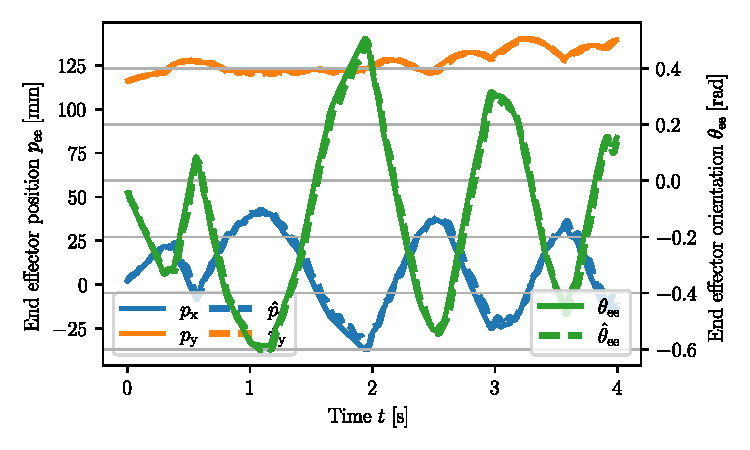
\includegraphics[width=0.48\columnwidth, trim={10, 10, 10, 10}]{hsamodel/figures/model_verification/20230621_183620_model_verification_chiee.pdf}\label{fig:hsamodel:planar_hsa_robot_model:model_verification:fpu:chiee}}
    \subfigure[FPU: Configuration]{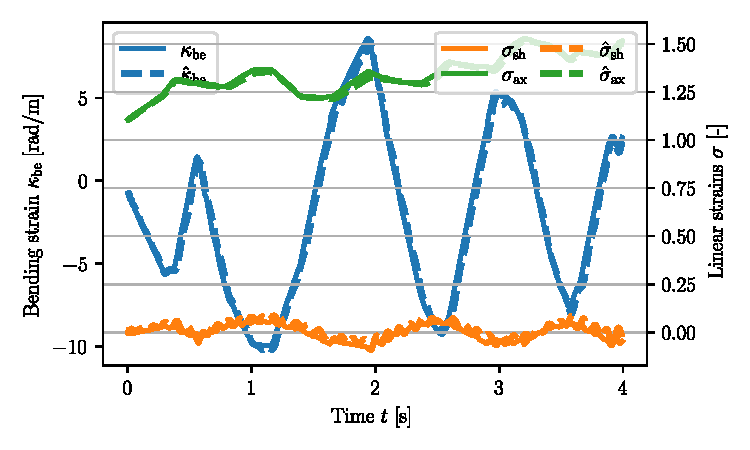
\includegraphics[width=0.48\columnwidth, trim={10, 10, 10, 10}]{hsamodel/figures/model_verification/20230621_183620_model_verification_q.pdf}\label{fig:hsamodel:planar_hsa_robot_model:model_verification:fpu:q}}\\
    \subfigure[EPU: End-effector pose]{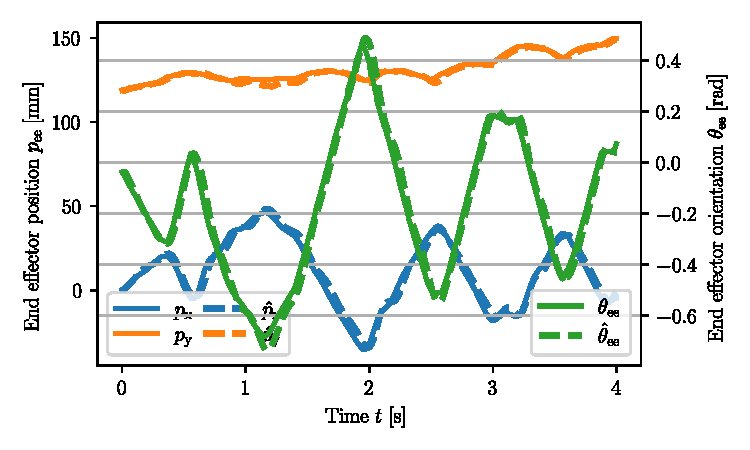
\includegraphics[width=0.48\columnwidth, trim={10, 10, 10, 10}]{hsamodel/figures/model_verification/20230927_150452_model_verification_chiee.pdf}\label{fig:hsamodel:planar_hsa_robot_model:model_verification:epu:chiee}}
    \subfigure[EPU: Configuration]{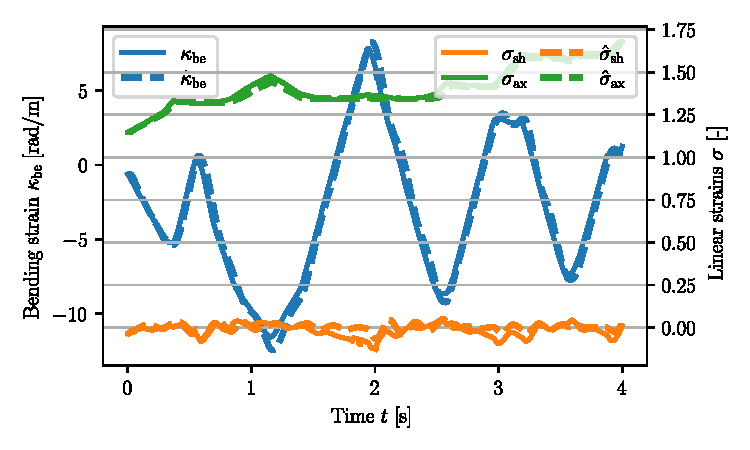
\includegraphics[width=0.48\columnwidth, trim={10, 10, 10, 10}]{hsamodel/figures/model_verification/20230927_150452_model_verification_q.pdf}\label{fig:hsamodel:planar_hsa_robot_model:model_verification:epu:q}}
    \caption{Verification of the system model and the identified system parameters on an unseen trajectory with the HSA being randomly actuated through a GBN sequence: the solid line denotes the actual trajectory. In contrast, the dashed line visualizes the trajectory simulated with the system model. We report results for both FPU and EPU-based \glspl{HSA}.}\label{fig:hsamodel:planar_hsa_robot_model:model_verification}
\end{figure}

\subsection{Model verification}\label{sub:hsamodel:planar_hsa_robot_model:model_verification}

\subsubsection{Experimental setup}\label{ssub:hsamodel:planar_hsa_robot_model:model_verification:experimental_setup}
We evaluate the planar \gls{HSA} model experimentally.
The material choice of the \gls{HSA} is crucial and has a significant influence on the resulting mechanical characteristics of the robot  (e.g., blocked force, holding torque, bending stiffness, etc.)~\citep{truby2021recipe}. Furthermore, specific material requirements are dictated by the nature of the design of the \gls{HSA} rod. The structure of the metamaterial is made of struts connected by living hinges. These living hinges must be thin, flexible, and accommodate high strains~\citep{truby2021recipe}.
In order to ensure that the system model is effective and suitable for a range of different materials, we decided to conduct the experimental verification on \glspl{HSA} 3D-printed via digital projection lithography either using the photopolymer resin Carbon FPU 50~\citep{carbon:fpu50} (stiffer) or the elastomeric polyurethane EPU 40 resin~\citep{carbon:epu40} (softer).

The Dynamixel MX-28 servo motor are set to use position control mode. % which runs a cascaded PID control loop on the motor current.
% The robot is mounted platform-down on a cage on which we have also attached eight Optitrack PrimeX 13 cameras. The motion capture system can track the SE(3) pose of both the base and the platform at a sampling rate of \SI{200}{Hz}. 
The robot is mounted platform-down on a cage with an Optitrack motion capture system, which measures the SE(3) pose of the platform at \SI{200}{Hz}.
Our algorithms run within a ROS2 framework\footnote{\url{https://github.com/tud-phi/ros2-hsa}}. % First, we project the pose measurements into the plane of actuation. Then, we evaluate the coordinate transformation between platform and base and run the closed-form inverse kinematics introduced in \eqref{eq:hsamodel:planar_hsa_robot_model:kinematics}. We store in memory the last \textcolor{orange}{ten} configuration measurements, fit a cubic spline to each configuration variable using the \emph{Derivative} package~\citep{kaptanoglu2022pysindy}, and then differentiate the spline function to gather $\dot{q}(t)$.
% ~\footnote{\url{https://github.com/tud-phi/ros2-hsa}}
% ~\citep{kaptanoglu2022pysindy}
% Our algorithms run within a ROS2 framework. 
The pose measurements are first projected into the plane of actuation and serve as an input to the closed-form inverse kinematics introduced in \eqref{eq:hsamodel:planar_hsa_robot_model:kinematics}. 
% We use a Savitzky-Golay filter with a window duration of $\SI{0.1}{s}$ to numerically differentiate $\chi_\mathrm{ee}(t)$, $q(t)$ and gather with that $\dot{\chi}_\mathrm{ee}(t)$ and $\dot{q}(t)$.
% We fit a cubic spline to the last $16$ configuration measurements and differentiate~\citep{kaptanoglu2022pysindy} to gather $\dot{q}(t)$.

\subsubsection{System identification}\label{ssub:hsamodel:planar_hsa_robot_model:model_verification:system_identification}
Next, we strive to identify the parameters used in our dynamic model.
We assume the robot's geometric and mass density properties to be known or easily measurable. % Therefore, we are left with having to identify the elastic and damping characteristics of the robot.
As knowledge about the damping coefficients is not required by the control law, only the experimental identification of elongation and stiffness characteristics remains.
For this, we measure the response of the system to step and staircase actuation sequences. Afterward, the parameters are regressed using least squares. % first in a static, pure elongation setting and then gradually also on dynamic sequences involving bending and shear.
For the FPU-based robot, we identify $C_\varepsilon^\mathrm{FPU}=\SI{0.0098}{m \per rad}$, $S_\mathrm{be}^\mathrm{FPU} = 0.00057 \cdot 10^{-5} - 9.7 \cdot 10^{-6} \, \frac{\phi_i^+}{l^0} \si{Nm^2}$, $S_\mathrm{sh}^\mathrm{FPU} = 0.591 - 0.00048 \, \frac{\phi_i^+}{l^0} \si{N}$, $S_\mathrm{ax}^\mathrm{FPU} = 5.665 + 0.0151 \, \frac{\phi_i^+}{l^0} \si{N}$, and $S_\mathrm{b,sh}^\mathrm{FPU} = 4.48 \cdot 10^{-3} \si{Nm \per rad}$ where $l^0 = \SI{0.059}{m}$. 
Furthermore, we regress $C_\varepsilon^\mathrm{EPU}=\SI{0.0079}{m \per rad}$, $S_\mathrm{be}^\mathrm{EPU} = -2.5 \cdot 10^{-5} + 3.9 \cdot 10^{-7} \, \frac{\phi_i^+}{l^0} \si{Nm^2}$, $S_\mathrm{sh}^\mathrm{EPU} = 0.0428 - 0.0029 \, \frac{\phi_i^+}{l^0} \si{N}$, $S_\mathrm{ax}^\mathrm{EPU} = 0.0 + 0.0098 \, \frac{\phi_i^+}{l^0} \si{N}$, and $S_\mathrm{b,sh}^\mathrm{EPU} = -\SI{0.0005}{Nm \per rad}$ for the EPU \glspl{HSA} which have the same length as the FPU \glspl{HSA}.
Finally, we identify the axial rest strain $\sigma_\mathrm{ax}^0$ before the start of each experiment.
We notice that the EPU-based HSA robot is approximately one order of magnitude more flexible than the FPU-based robot.

\subsubsection{Results}\label{ssub:hsamodel:planar_hsa_robot_model:model_verification:results}
We verify the accuracy of the proposed system model and the identified parameters on trajectories unseen during system identification. We generate the trajectories by actuating the robot with a \gls{GBN}~\citep{tulleken1990generalized} sequence with a settling time of \SI{0.5}{s} and at each time step $k$ randomly sample $\phi(k) \sim \mathcal{U}(0, \phi_\mathrm{max})$.
We simulate the model evolution with a Dormand-Prince 5(4) integrator and a time step of \SI{0.1}{ms}.
Fig.~\ref{fig:hsamodel:planar_hsa_robot_model:model_verification:fpu:chiee} shows the model exhibiting excellent accuracy for representing the behavior of FPU-based \gls{HSA} robots.
We observe more significant errors in the shear estimate for EPU-based \gls{HSA} robots in Fig.\ref{fig:hsamodel:planar_hsa_robot_model:model_verification:epu:q}. Specifically, the \gls{CS} model no longer seems sufficient for capturing the robot's shape, particularly for larger bending angles. Therefore, we suggest for future work to employ kinematic models with more \gls{DOF} such as \gls{PCS} as proposed, for example, in Sec.~\ref{sec:hsamodel:hsa_rod_kinematics} or \citep{renda2018discrete}.
